\documentclass[10pt]{article}
\usepackage[margin=1in]{geometry}
\usepackage{CJKutf8}
\usepackage{booktabs}
\usepackage{array}
\usepackage{graphicx}
\usepackage{amsmath}
\usepackage{microtype}
\usepackage[unicode,hidelinks,pdftitle={Knowing When You Do Not Know Where: Selective, Registry-Verified Municipality Resolution for Japanese Addresses},pdfauthor={Sushil Raj}]{hyperref}
\usepackage{url}

\title{Knowing When You Do Not Know Where:\\Selective, Registry-Verified Municipality Resolution\\for Japanese Addresses}
\author{Sushil Raj\\\texttt{sushilraj0177@gmail.com}}
\date{November 2026}

\begin{document}
\begin{CJK}{UTF8}{min}
\maketitle

\begin{abstract}
About one in twenty hand-typed Japanese addresses leaves out its municipality, and the district name
that remains often exists in many municipalities. Tools that always answer turn this into silent
errors. We treat municipality resolution as selective prediction: JADEN, an offline open-source
engine, checks each reading against official gazetteers and declines when several municipalities
remain, and a calibrated scorer adds probabilities, a risk-controlled answer threshold and conformal
candidate sets. In two pre-registered tests on data never used in development (321,859 welfare and
206,041 medical facilities), JADEN's rules answered about half of the district-only inputs and were
wrong on 0.38\% and 0.28\% of their answers; jageocoder answered about three quarters correctly but
was wrong on 21--23\% of its answers. After the tests, a jageocoder that declines when its best matches
span several municipalities answered 73--76\% at 3--4\% wrong, beating JADEN's resolver at equal coverage
(5--8\%): JADEN's advantage is a controllable operating point near 1\% wrong with calibrated
probabilities, not better ranking. The calibrated resolver answered 59--61\% at
0.72--1.14\% wrong; its 1\% target held in one test and failed in the other (1.10\%), and conformal
coverage fell about 1.2 points short of 95\% in both. A language model choosing from JADEN's
candidates was wrong on 31.6\% of its answers. Of 13 pre-registered hypotheses, 7 held. In two further
pre-registered studies, the municipality codes of four public registers (5.8 million records) contradicted
an address that writes its municipality in under 0.07\% of records, mostly through a wrong code
where locations could tell; and on 9,878 addresses written with municipalities that no longer
exist, JADEN named today's municipality for 91--99\% at 0.07--1.0\% wrong, jageocoder for 83--86\% at
9.5--10\% wrong. Code, protocols, logs and results are public.
\end{abstract}

% ------------------------------------------------------------------------------------------
\section{Introduction}

A Japanese address names, from the largest unit down, a prefecture (都道府県), a municipality (市区町村;
in the 20 designated cities, a ward), a district (町字, \emph{machiaza}, such as 錦町 or 栄町 or 芝公園)
with an optional 丁目 subdivision, and block and building numbers. In practice the upper levels are often
left out. In the register of long-term-care offices published by the Ministry of Health, Labour and
Welfare, 13.5\% of the addresses typed by the offices themselves leave out the prefecture and 5.1\% the
municipality (Section~\ref{sec:prevalence}); MLIT publishes every welfare-facility address without it.
District names repeat across the country: 錦町 is a district in 93 municipalities, and 栄町 is both a
municipality in Chiba and a district in 224 other municipalities. Between 1999 and 2010, mergers cut the
number of municipalities from about 3,200 to about 1,700, so older records also carry names that no
longer exist.

For an address without its municipality, a resolver must either pick one of the places the district
name could mean or say that it cannot tell. Most tools pick. When records are linked to municipalities
in bulk (for subsidies, inspections or statistics), a wrong pick is silent. We study the other
option: \emph{selective} resolution, which answers only when the evidence settles the municipality, says
how sure it is, and returns the remaining candidates otherwise.

\paragraph{Contributions.}
\begin{enumerate}
\item \textbf{Registry-verified selective resolution} (Section~\ref{sec:method}). A rule engine that keeps
every municipality where the written district exists and removes candidates only by registry facts,
and a conditional-logit scorer with a ``none of these'' option on top of it, with a risk-controlled
answer threshold and split-conformal candidate sets.
\item \textbf{Two pre-registered held-out tests} (Sections~\ref{sec:protocol}--\ref{sec:results}). For each,
the question, frozen test files, systems, measures and directional hypotheses were committed to the
public repository before any system ran on the test data, and results are reported as they came out.
The second test also measures whether ten rounds of rule fixes made between the tests generalised.
\item \textbf{Analyses made after the tests, reported as such} (Section~\ref{sec:posthoc}): a comparison
with jageocoder on equal terms, which shows that JADEN's advantage lies in calibrated selectivity rather
than in ranking; a corrected calibration procedure; a check for leakage through the prior; and intervals
that respect repeated addresses.
\item \textbf{Language models in the loop} (Section~\ref{sec:llmres}): choosing from a verified candidate
list does not make a model reliable; checking its free answers against the registry removes most of its
errors, though part of that effect comes from a confidence filter.
\item \textbf{Two applications, each pre-registered} (Section~\ref{sec:studies}): an audit of 5.8 million
records of four public registers for codes that contradict their own addresses, and the resolution of
addresses written with municipalities that have since been merged or renamed, both scored against
surveyed locations rather than text.
\end{enumerate}
JADEN (MIT licence) has no runtime dependencies and needs no network access. All code, protocols, run
logs and result files are in the repository (Section~\ref{sec:repro}).

% ------------------------------------------------------------------------------------------
\section{Related work}

\paragraph{Japanese address infrastructure and tools.} The Digital Agency maintains the Address Base
Registry (アドレス・ベース・レジストリ, ABR) with a master of districts (町字マスター) and publishes an
open-source geocoder for it, \texttt{abr-geocoder} \cite{abr}. The Center for Spatial Information Science
at the University of Tokyo has long offered CSV address matching against MLIT's location reference data
\cite{csis}; its output includes a confidence level (iConf) that marks addresses whose place names are
unique at two or more levels. jageocoder \cite{jageocoder}, by the same developer, returns every node whose
match is equally good, so ambiguity is visible to the caller; Geolonia's normalize-japanese-addresses
\cite{geolonia} returns one normalised reading. The GeoNLP project \cite{geonlp} provides place-name
dictionaries and geotagging for Japanese text. Hisamoto et al.\ \cite{hisamoto} survey geocoding as the
disambiguation of place references, and historical address geocoding has been built for Meiji-era Tokyo
\cite{ishikawa}. What these tools do not provide is a probability with a stated error rate for the
municipality when the address does not name it; that is the gap this paper addresses.

\paragraph{Toponym resolution and record linkage.} Resolving an ambiguous place name to one referent is
toponym resolution \cite{leidner}; population or frequency priors are a standard signal, and evaluation
practice has been surveyed critically \cite{gritta}. For Japanese, ATD-MCL annotates geo-entity
mentions, coreference and database links in travelogues \cite{atdmcl}. Our town-frequency prior is such a
signal, counted from registered corporations. Deciding whether two records refer to the same place is
record linkage \cite{fellegi}, the setting in which address resolution is usually deployed.

\paragraph{Geocoding and language models.} End-to-end systems generate coordinates directly
\cite{reageo} or ground compositional location references with an LLM and a geoparser's knowledge base
\cite{masis}. MESSY STREETS \cite{messy} finds that the gap between commercial and open-source geocoders
on messy real addresses comes mostly from returning no candidate at all, and GeoHaluBench \cite{geohalu}
shows that LLMs hallucinate geographic facts. AddrKG-LLM \cite{addrkg} retrieves candidate communities
with a knowledge graph and lets an on-premise LLM choose only among them.

\paragraph{Selective prediction and calibration.} Reject options go back to Chow \cite{chow}; selective
classification with guaranteed risk \cite{geifman} and Learn-then-Test \cite{ltt} choose thresholds whose
risk is controlled with high probability. Temperature scaling \cite{guo} calibrates a scorer with one
parameter. Split conformal prediction \cite{vovk,angelopoulos} gives prediction sets with marginal
coverage under exchangeability, and pipeline versions extend it to multi-stage language systems
\cite{pasc}. Exchangeability is exactly what breaks when calibration and test data come from different
publishers, which our tests measure.

% ------------------------------------------------------------------------------------------
\section{Method}\label{sec:method}

\subsection{The rule engine}
JADEN parses an address into prefecture, municipality, district, 丁目 and block numbers and checks each
against official data: the MIC list of municipality codes (1,918 entries including designated-city
wards), MLIT's 大字・町丁目レベル位置参照情報 (a gazetteer of 191,100 districts and 丁目 with
representative points), Japan Post's postal-code list and 1,829 former municipality names. The gazetteer
is not complete: some local names in use are missing from it. When the municipality is missing, every
municipality where the written district exists becomes a candidate; candidates are removed only by
registry facts (the written 丁目 does not exist there, the postal code belongs elsewhere). One survivor
is \textsc{accepted}; several are \textsc{ambiguous}, with the list.

The rules were developed on two registers, which are therefore \emph{development} results, not
evaluations: on the 5,049,462 active corporations of the National Tax Agency register, the rules name
the row's municipality for 99.98\% of full addresses (6 wrong, each a row whose own code contradicts its
address); on the 223,161 care-office addresses as typed, 97.88\% (13 wrong), and 99.87\% (4 wrong) once
the row's prefecture and municipality columns are put in front.

\subsection{Calibrated resolution}
\paragraph{Candidates and evidence.} The candidates of an input are JADEN's accepted municipality or its
ambiguous list; very long lists are cut to 60, keeping municipalities whose own name is written and then
the districts with the most corporations. Each candidate $c$ gets a feature vector $x_c$: the number of
corporations registered in the matched district there (log) and its share among the candidates; the
number in the municipality (log); whether the district and the written 丁目 exist there; whether the
rules accepted it or the municipality was written; whether its name is used in the input as a district
name; and, when given, whether the organisation's name mentions the municipality or the prefecture. A
vector $g$ describes the evidence that the answer is none of the candidates.

\paragraph{Model.} A conditional logit with an outside option:
\begin{equation}
P(c) = \frac{e^{w\cdot x_c}}{Z},\qquad P(\text{none}) = \frac{e^{v\cdot g}}{Z},\qquad
Z = \sum_{c} e^{w\cdot x_c} + e^{v\cdot g}.
\end{equation}
The outside option matters because the gazetteer is incomplete: a single candidate is not certain.
Parameters are fitted by maximum likelihood (L-BFGS, L2 penalty $10^{-3}$) on 359,994 inputs built
from 120,000 sampled corporation addresses (the district part alone, prefecture plus district part, and
the full address, each with the corporation's name). The prior counts the 4,977,458 corporations
registered in each of 107,653 districts, leaving each training row's own corporation out.

\paragraph{Calibration.} The care offices are split in half by office number. On the calibration half
(304,137 inputs) a single temperature is fitted; the answer threshold $\tau$ is the lowest probability
for which, for each input type, the 95\% Clopper--Pearson upper bound of the wrong-answer rate among
answers with $p \ge \tau$ is at most 1\% ($\tau = 0.882$; 0.878 with the name); conformal quantiles
$\hat q$ per input type give sets $\{c : 1 - P(c) \le \hat q\}$ meant to hold the right option, possibly
``none'', 95\% of the time. The other half (305,913 inputs) is a development check. Two weaknesses of
this procedure, found after the tests, are analysed in Section~\ref{sec:recal}.

\paragraph{A change between the tests.} After test~1, a defect in the name feature was fixed: the
prefecture-mention check matched 京都 inside 東京都. The model's weights were not refitted, so test~2 ran
the corrected feature with the weights fitted on the defective one.

\subsection{Language models in the loop}\label{sec:llm}
\begin{sloppypar}
For town-only inputs the calibrated resolver with the name does not answer, a language model
(\texttt{claude-haiku-5-5}, and \texttt{claude-sonnet-5-5} in the
amendment, called through the Claude
Code command line in November 2026 with default settings, 20 addresses per call) receives the address
and the facility's name. \emph{Choose}: JADEN's candidates are listed and the model returns one or
declines, with a confidence. \emph{Propose and verify}: the model names the municipality freely; the
answer is kept only if it is one of JADEN's candidates and the model states a confidence of at least 80.
\emph{Alone}: the free answer, unverified. A development trial on 400 ambiguous care addresses, run before
any test call, motivated propose-and-verify; it was added to the first protocol as a dated amendment.
Prompts and raw answers are in the repository.
\end{sloppypar}

% ------------------------------------------------------------------------------------------
\section{Evaluation protocol}\label{sec:protocol}

\begin{table}[t]
\centering\small
\begin{tabular}{@{}llr@{}}
\toprule
Role & Data & Size \\
\midrule
Prior and training & National Tax Agency corporation register (2026-10-30) & 5,049,462 corporations \\
Calibration / check & MHLW care-office register (June 2026), split by office number & 304,137 / 305,913 inputs \\
Rule development & both of the above, and JA-AddrBench (4,700 school addresses) & \\
\textbf{Test 1} & \textbf{MLIT 国土数値情報 welfare facilities P14 (2023)} & \textbf{321,859 facilities} \\
\textbf{Test 2} & \textbf{MHLW 医療情報ネット medical facilities (2026-06-01)} & \textbf{206,043 facilities} \\
\bottomrule
\end{tabular}
\caption{Data. For test 2, the development data also include test 1's file. Both test files are frozen by
their full SHA-256 in the protocols.}
\label{tab:data}
\end{table}

Both tests follow the same rules (Table~\ref{tab:data}). A protocol stating the question, the frozen test
files, the systems, the measures and directional hypotheses is committed to the public repository before
any system runs on the test data; commit times, the times each run started and ended, and the run logs
are published with the results. No test row is used for training, calibration, thresholds or code
changes before the results are written; each test is run once, and every deviation (tool concurrency, a
retry of 50 network failures of one tool) is listed with the results. An answer is right when it names
the row's municipality or a ward of the row's designated city. The input that holds only the district
and what follows it is called ``town only'', as in the protocols.

\paragraph{Test 1} (protocol of 19 November 2026). MLIT publishes welfare-facility addresses
\emph{without} the municipality, with the municipality code alongside. Each facility gives a town-only
input (the address as published), a prefecture-plus-address input and a full input; the facility name
is side information. 318,578 facilities carry a code that is still current and are scored. Because the
welfare file's largest category includes care facilities that may also be in the development data,
results are also reported for the categories that cannot be care offices (59,503 facilities). The
language-model systems run on random samples of 1,000 inputs.

\paragraph{Test 2} (protocol of 25 November 2026). The medical-facility tables give addresses typed by the
facilities themselves, with the municipality. Inputs are the full address as published, the address
without the prefecture, and the address with prefecture, county and municipality stripped (so the
town-only inputs of this test are derived, not observed). The engine at the test~1 commit runs on the same
inputs. Results are also reported for the 180,655 facilities whose full address, after Unicode
normalisation and removal of spaces, matches no development address; this catches only exact repeats.
No language model is run.

% ------------------------------------------------------------------------------------------
\section{Results}\label{sec:results}

\begin{table}[t]
\centering\footnotesize\setlength{\tabcolsep}{4pt}
\resizebox{\linewidth}{!}{\begin{tabular}{@{}llrrrlrl@{}}
\toprule
Input & System & Answered & Right & Wrong & Wrong among answers (95\% CI) & ECE & Conformal cov.\ / size \\
\midrule
town only & JADEN rules & 52.36\% & 52.16\% & 639 & 0.38\% (0.35--0.41) & -- & -- \\
 & JADEN calibrated & 60.44\% & 59.78\% & 2,115 & 1.10\% (1.05--1.15) & 0.015 & 93.72\% / 2.39 \\
 & JADEN calibrated + name & 61.91\% & 61.20\% & 2,255 & 1.14\% (1.10--1.19) & 0.007 & 93.83\% / 2.16 \\
 & jageocoder & 97.23\% & 76.46\% & 66,164 & 21.36\% (21.22--21.50) & -- & -- \\
 & Geolonia & 2.00\% & 0.03\% & 6,256 & 98.40\% (98.06--98.68) & -- & -- \\
\midrule
with prefecture & JADEN rules & 81.45\% & 81.33\% & 374 & 0.14\% (0.13--0.16) & -- & -- \\
 & JADEN calibrated + name & 87.18\% & 86.93\% & 799 & 0.29\% (0.27--0.31) & 0.004 & 94.11\% / 0.96 \\
 & jageocoder & 4.01\% & 2.51\% & 4,758 & 37.28\% (36.44--38.12) & -- & -- \\
 & Geolonia & 0.09\% & 0.03\% & 194 & 64.67\% (59.10--69.86) & -- & -- \\
\midrule
full & JADEN rules & 99.98\% & 99.98\% & 0 & 0.00\% & -- & -- \\
 & jageocoder & 100.00\% & 100.00\% & 0 & 0.00\% & -- & -- \\
 & Geolonia & 100.00\% & 100.00\% & 0 & 0.00\% & -- & -- \\
\bottomrule
\end{tabular}}
\caption{Test 1 (318,578 facilities per input type). Answered and right are shares of all inputs; wrong is
a count.}
\label{tab:test1}
\end{table}

\begin{table}[t]
\centering\footnotesize\setlength{\tabcolsep}{4pt}
\resizebox{\linewidth}{!}{\begin{tabular}{@{}llrrrlrl@{}}
\toprule
Input & System & Answered & Right & Wrong & Wrong among answers (95\% CI) & ECE & Conformal cov.\ / size \\
\midrule
full & JADEN rules (final) & 99.95\% & 99.95\% & 0 & 0.000\% (0.000--0.002) & -- & -- \\
 & JADEN rules (test 1 engine) & 99.95\% & 99.95\% & 0 & 0.000\% (0.000--0.002) & -- & -- \\
 & jageocoder & 99.97\% & 99.97\% & 0 & 0.000\% (0.000--0.002) & -- & -- \\
 & Geolonia & 99.99\% & 99.99\% & 0 & 0.000\% (0.000--0.002) & -- & -- \\
\midrule
no prefecture & JADEN rules (final) & 99.87\% & 99.87\% & 0 & 0.000\% (0.000--0.002) & -- & -- \\
 & JADEN rules (test 1 engine) & 99.88\% & 99.88\% & 0 & 0.000\% (0.000--0.002) & -- & -- \\
 & jageocoder & 99.97\% & 99.97\% & 2 & 0.001\% (0.000--0.004) & -- & -- \\
 & Geolonia & 99.99\% & 99.97\% & 50 & 0.024\% (0.018--0.032) & -- & -- \\
\midrule
town only & JADEN rules (final) & 48.93\% & 48.80\% & 279 & 0.28\% (0.25--0.31) & -- & -- \\
 & JADEN rules (test 1 engine) & 49.22\% & 48.85\% & 774 & 0.76\% (0.71--0.82) & -- & -- \\
 & JADEN calibrated & 59.01\% & 58.59\% & 880 & 0.72\% (0.68--0.77) & 0.006 & 93.77\% / 2.33 \\
 & JADEN calibrated + name & 60.32\% & 59.80\% & 1,075 & 0.87\% (0.82--0.92) & 0.005 & 93.72\% / 2.12 \\
 & jageocoder & 97.83\% & 75.80\% & 45,343 & 22.52\% (22.34--22.70) & -- & -- \\
 & Geolonia & 2.19\% & 0.06\% & 4,385 & 97.47\% (96.97--97.89) & -- & -- \\
\bottomrule
\end{tabular}}
\caption{Test 2 (206,041 facilities; 205,830 town-only inputs). On the 180,655 unseen facilities the final
rules are wrong on 0\% of full and prefecture-less answers and on 0.30\% (0.26--0.33) of town-only
answers.}
\label{tab:test2}
\end{table}

\subsection{Both tests}
Tables~\ref{tab:test1} and~\ref{tab:test2} show the same pattern on two publishers' data. With the full
address, every tool is right on essentially every input; JADEN declines slightly more often (0.05\% in
test~2) and is never wrong. Without the prefecture (test~2), Geolonia's 50 wrong answers are all
municipality names that exist in two prefectures (府中市: Tokyo or Hiroshima; 伊達市: Hokkaido or
Fukushima). With only the district, the tools separate. jageocoder answers almost every input and is
right on about three quarters of all inputs, far more than JADEN's 49--62\%; it is also wrong on 21--23\%
of the inputs it answers. JADEN's rules answer about half and are wrong on 0.28--0.38\% of those. These
are different operating points, and comparing wrong-answer counts alone flatters the tool that declines;
Section~\ref{sec:fair} compares them on equal terms. Geolonia is not designed for district-only input and
answers almost none of it.

The calibrated resolver answers 8--11 points more than the rules. Its threshold, chosen on care-office
data for a 1\% wrong-answer rate, gave 1.10\% (1.05--1.15) in test~1 and 0.72\% (0.68--0.77) in test~2.
Its probabilities stay well calibrated (ECE 0.005--0.015), but conformal sets meant to cover 95\% covered
93.7--93.8\% in both tests. JADEN's offline points lie a median 165\,m (丁目 level) and 380\,m
(district level) from the medical publisher's own coordinates.

\subsection{Language models (test 1)}\label{sec:llmres}

\begin{table}[t]
\centering\footnotesize\setlength{\tabcolsep}{4pt}
\resizebox{\linewidth}{!}{\begin{tabular}{@{}llrll@{}}
\toprule
System & Filter on the model's answers & Kept & Wrong among kept (95\% CI) & Right answers discarded \\
\midrule
Haiku chooses from the list (remainder) & none (system 4) & 526 & 166 (27.7--35.7\%) & -- \\
 & confidence $\ge 80$ & 337 & 70 (16.8--25.4\%) & 93 \\
Haiku proposes (remainder) & none & 478 & 184 (34.2--42.9\%) & -- \\
 & confidence $\ge 80$ & 180 & 13 (4.3--12.0\%) & 127 \\
 & in JADEN's candidates & 358 & 70 (15.8--24.0\%) & 6 \\
 & both (system 4b) & 172 & 10 (3.2--10.4\%) & 132 \\
Sonnet proposes (remainder) & none & 851 & 399 (43.6--50.2\%) & -- \\
 & confidence $\ge 80$ & 339 & 38 (8.3--15.0\%) & 151 \\
 & in JADEN's candidates & 485 & 41 (6.3--11.3\%) & 8 \\
 & both (system 4b) & 303 & 8 (1.3--5.1\%) & 157 \\
Haiku alone (random) & none (system 5) & 624 & 166 (23.3--30.2\%) & -- \\
Sonnet alone (random) & none (system 5) & 957 & 340 (32.6--38.6\%) & -- \\
\bottomrule
\end{tabular}}
\caption{Language models on the 1,000-input samples of test 1. ``Remainder'': town-only inputs the
calibrated resolver with the name leaves unanswered; ``random'': random town-only inputs. Rows with a
filter other than ``none'' and the pre-registered system rows (choose; propose with both filters) are
separated here to show what each filter does; only the latter were pre-registered.}
\label{tab:llm}
\end{table}

Table~\ref{tab:llm}. Given JADEN's list, Haiku answered 526 of the 1,000 remainder inputs and was wrong on
166 (31.6\%); answering freely on random inputs, it was wrong on 26.6\%, so the list did not make it more
reliable. Keeping only free answers that are among JADEN's candidates removes most wrong answers; adding
the confidence filter, which the choose system did not get, removes more but also discards many right
answers. The comparison that isolates verification is the row ``in JADEN's candidates'': for Sonnet it keeps 485 of 851 answers with 41 wrong (8.5\%) and discards only 8 right
ones; for Haiku, 358 of 478 with 70 wrong (19.6\%). With the same confidence filter, choosing from the list
left 20.8\% wrong (337 kept) while proposing freely left 7.2\% (180 kept), so the list itself made the
answers worse, not only the missing filter. Adding verified Sonnet proposals to the calibrated resolver
would answer a projected 71.7\% of test~1's town-only inputs at 1.36\% wrong among answers (from the
113,057 inputs left with candidates).
Free answers also named municipalities that no longer exist (茶屋町, merged into 倉敷市 in 2005;
浜松市中区, abolished in 2024): 2 to 6 in each 1,000-input sample.

\subsection{Hypotheses}

\begin{table}[t]
\centering\small
\begin{tabular}{@{}l>{\raggedright\arraybackslash}p{0.5\linewidth}>{\raggedright\arraybackslash}p{0.35\linewidth}@{}}
\toprule
& Pre-registered statement & Result \\
\midrule
1-H1 & Rules give fewer wrong town-only answers than jageocoder and Geolonia & \textbf{Held}: 639 vs 66,164 and 6,256 \\
1-H2 & Calibration transfers: ECE $\le 0.03$ & \textbf{Held}: 0.015 (0.007 with name) \\
1-H3 & The 1\% threshold's wrong-answer rate has a 95\% interval including or below 1\% & \textbf{Failed}: 1.10\% (1.05--1.15). On the categories that cannot be care offices: 1.02\% (0.92--1.13) \\
1-H4 & Calibrated answers more than rules; the name adds more & \textbf{Held}: +7.6 points, +1.4 with name \\
1-H5 & Conformal 95\% sets cover $\ge 95\%$ & \textbf{Failed}: 93.7\% \\
1-H6 & Choosing from JADEN's list: wrong on $<5\%$ of answers; alone, the model is wrong more often and names municipalities that do not exist & \textbf{Failed}: 31.6\% wrong when choosing; alone, Haiku was wrong less often (26.6\%), though it named 6 non-existent municipalities \\
1-H7 & (amendment) Propose and verify: upper bound $\le 10\%$; most free errors removed & \textbf{Held for Sonnet} (2.6\%, bound 5.1\%); \textbf{failed for Haiku} (5.8\%, bound 10.4\%) \\
\midrule
2-H1 & Full addresses: rules answer $\ge 99.5\%$; wrong-rate bound $\le 0.05\%$ & \textbf{Held}: 99.95\%, 0 wrong (bound 0.002\%) \\
2-H2 & No prefecture: bound $\le 0.1\%$; fewer wrong than both other tools & \textbf{Held}: 0 vs 50 and 2 \\
2-H3 & Town only: bound $\le 0.5\%$; fewer wrong than both other tools & \textbf{Held}: 0.28\% (0.25--0.31); 279 vs 45,343 and 4,385 \\
2-H4 & The 1\% threshold's interval includes or lies below 1\% & \textbf{Held}: 0.72\% (0.68--0.77) \\
2-H5 & Conformal 95\% sets cover $\ge 95\%$ & \textbf{Failed}: 93.8\% \\
2-H6 & The rule fixes generalise: on full and prefecture-less input, no more wrong and no fewer right answers & \textbf{Failed}: 0 wrong in both, but 17 fewer right of 206,041 \\
\bottomrule
\end{tabular}
\caption{Pre-registered hypotheses and outcomes: 7 held, 1 held for one model and failed for the other,
5 failed. 1-H1, 2-H2 and 2-H3 compare wrong-answer counts between a tool that declines and tools that
answer almost everything; Section~\ref{sec:fair} compares them on equal terms.}
\label{tab:hyp}
\end{table}

Table~\ref{tab:hyp} lists every pre-registered hypothesis. Hypotheses that compare wrong-answer counts with
tools that rarely decline (1-H1, 2-H2, 2-H3) were close to guaranteed by design; the informative ones are
those about calibration, error control and coverage (1-H2, 1-H3, 1-H5, 2-H4, 2-H5), and three of those five
failed.

% ------------------------------------------------------------------------------------------
\section{Analyses after the tests}\label{sec:posthoc}

The analyses in this section were not pre-registered. They were made after both tests, in response to a
critical review, from the stored outputs of the tests or by rerunning a system on the same frozen inputs.

\subsection{JADEN and jageocoder on equal terms}\label{sec:fair}
The pre-registered comparison scored jageocoder's first answer for every input, so it mixes two
differences: how well a tool ranks the candidates, and whether it may decline. jageocoder returns every
equally good match; a jageocoder that answers only when all of them lie in one municipality is the
simplest abstaining version its own output allows. We ran it, and JADEN's calibrated resolver made to
answer the same share of inputs (highest probabilities first), on random samples of 40,000 town-only
inputs per test (seed 2026; Table~\ref{tab:fair}, Figure~\ref{fig:fair}).

\begin{figure}[t]
\centering
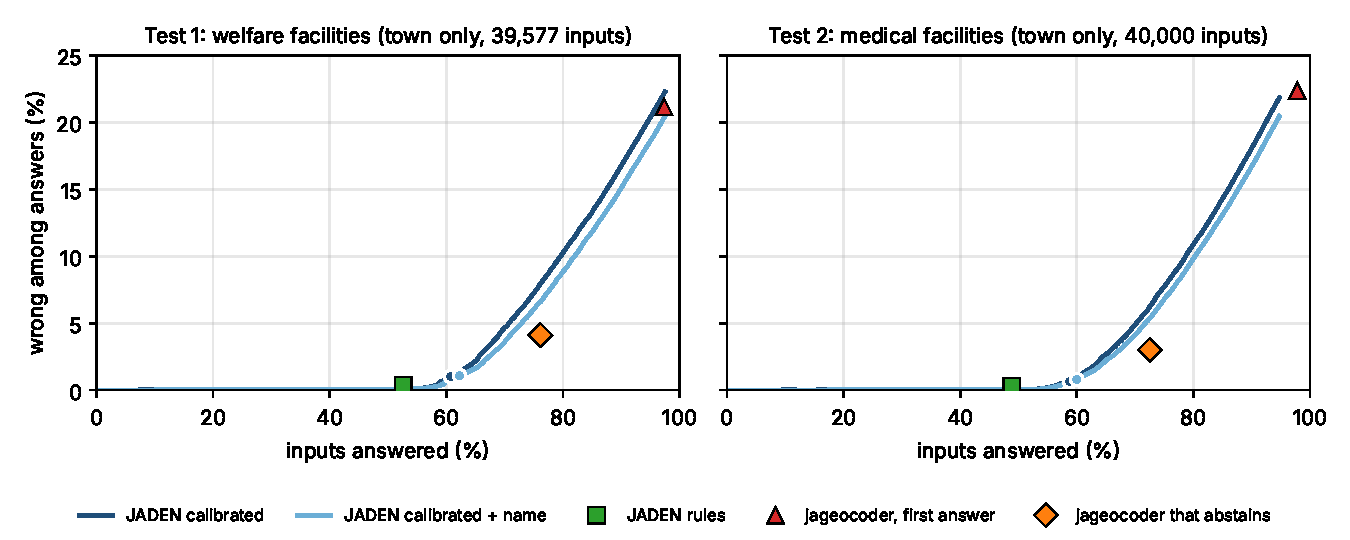
\includegraphics[width=\linewidth]{fair_curves.pdf}
\caption{Wrong-answer rate among answers against the share of town-only inputs answered (post hoc, same
samples as Table~\ref{tab:fair}). Curves: JADEN's calibrated resolver answering the most probable inputs
first, with its threshold marked by a dot. Points: JADEN's rules and the two jageocoder variants.}
\label{fig:fair}
\end{figure}

\begin{table}[t]
\centering\footnotesize\setlength{\tabcolsep}{4pt}
\begin{tabular}{@{}lrrrrrr@{}}
\toprule
& \multicolumn{3}{c}{Test 1 (39,577 inputs)} & \multicolumn{3}{c}{Test 2 (40,000 inputs)} \\
System & Answered & Right & Wrong/ans. & Answered & Right & Wrong/ans. \\
\midrule
jageocoder, first answer & 97.3\% & 76.8\% & 21.1\% & 97.8\% & 75.9\% & 22.4\% \\
jageocoder that abstains & 76.1\% & 73.0\% & \textbf{4.1\%} & 72.5\% & 70.4\% & \textbf{3.0\%} \\
JADEN rules & 52.6\% & 52.4\% & 0.34\% & 48.9\% & 48.7\% & 0.27\% \\
JADEN calibrated, at its threshold & 60.7\% & 60.1\% & 1.0\% & 58.8\% & 58.4\% & 0.65\% \\
\quad answering as many as the abstaining jageocoder & 76.1\% & 70.1\% & 7.9\% & 72.5\% & 68.0\% & 6.3\% \\
\quad answering as many as jageocoder's first answer & 97.3\% & 75.8\% & 22.1\% & 94.7\% & 74.0\% & 21.8\% \\
JADEN calibrated + name, at its threshold & 62.3\% & 61.6\% & 1.1\% & 60.0\% & 59.5\% & 0.80\% \\
\quad answering as many as the abstaining jageocoder & 76.1\% & 71.1\% & 6.6\% & 72.5\% & 68.6\% & 5.4\% \\
\quad answering as many as jageocoder's first answer & 97.3\% & 77.5\% & 20.3\% & 94.7\% & 75.4\% & 20.4\% \\
\bottomrule
\end{tabular}
\caption{Town-only input on equal terms (post hoc). ``Answering as many as'' lets JADEN answer the same
share of inputs, most probable first; in test 2 JADEN has candidates for only 94.7\% of the sample.}
\label{tab:fair}
\end{table}

The result is not in JADEN's favour. The abstaining jageocoder answers 76.1\% (test~1) and 72.5\% (test~2)
of the inputs with 4.1\% and 3.0\% wrong; JADEN's calibrated resolver made to answer as many is wrong on
7.9\% and 6.3\% (6.6\% and 5.4\% with the name). Answering everything, the two are about equal. What JADEN
adds is an operating point near 1\% wrong (about 60\% answered) and a probability for every answer, which
lets a user choose that point; at the coverage where jageocoder's own abstention rule operates,
jageocoder is more accurate. A likely reason is the data. jageocoder's dictionary goes down to blocks
(街区), so a district name followed by block numbers matches only where that block exists; JADEN's bundled
gazetteer stops at 丁目, and its optional block data is consulted only after a single municipality has been
chosen, never to eliminate candidates. Eliminating candidates whose block does not exist is the clearest
improvement this comparison points to. We do not tune it on these tests; it needs a new pre-registered
test.

\subsection{A corrected calibration procedure}\label{sec:recal}
The pre-registered calibration had two flaws. Its threshold search scanned thresholds from low to high and
kept the first whose bound passed, with no control for testing many thresholds; and the temperature, the
threshold and the conformal quantiles were all fitted on the same half of the care data, while split
conformal coverage assumes the quantile is computed on data not used to fit the scores. We redid the
calibration step with the model's weights unchanged: the temperature on one half of the calibration data
(split by facility), and on the other half the conformal quantiles and the threshold, found by
fixed-sequence testing from the strictest threshold down (Learn-then-Test \cite{ltt}), stopping at the first
threshold whose 95\% bound exceeds 1\% for any input type. The sequence starts where every input type has
1,000 answers, a choice made from the scores alone. The corrected thresholds are close to the
pre-registered ones (0.873 against 0.882; 0.877 against 0.878 with the name), and so are the results: on
the care development check the town-only wrong-answer rate is 1.02\% (0.94--1.09), on test~1 1.20\%
(1.15--1.24) and on test~2 0.89\% (0.84--0.94), with conformal coverage of 93.6--93.7\% on both tests. The
error control holds on data like its calibration data and does not carry over exactly to other
publishers; the corrected procedure does not change that.

\subsection{Leakage through the prior}
The prior counts every corporation in the National Tax Agency register, including operators registered
at a test facility's own address (a medical corporation at its clinic), whose count favours exactly the
right municipality. Matching corporations to test facilities by municipality, district and the full
number sequence (a strict match that also catches other tenants of the same building) found 196,451
corporations sharing a key with 189,019 of the 524,408 test facilities. Removing them from the prior and
rebuilding every town-only input changed little: in test~2 the calibrated resolver's wrong-answer rate went
from 0.72\% to 0.75\% and its right answers from 58.59\% to 58.50\% (with the name, 0.87\% and 59.80\% to
0.87\% and 59.73\%); in test~1, rebuilt with the current engine, from 0.76\% to 0.78\%. The prior's value
does not come from the facilities' own operators.

\subsection{Repeated addresses}
Several facilities can share one address (clinics in one building), so the inputs are not independent.
A bootstrap over clusters of identical input texts widens the intervals only slightly: test~1 rules 0.35--0.42\% (Wilson 0.36--0.41\%) and
calibrated 1.04--1.16\% (1.05--1.15\%); test~2 rules 0.22--0.36\% (0.25--0.31\%) and calibrated
0.68--0.77\% (unchanged). No conclusion changes; test~1's calibrated interval still excludes 1\%.

\subsection{Did the rule fixes overfit?}
Between the tests the rules went through ten rounds of fixes found by reviewing failures on development
data. On test~2's inputs, the fixes cut town-only wrong answers from 774 to 279 (484 became no answer, 11
became right), at a cost of 138 right answers that became no answer. On full and prefecture-less input
both engines make no wrong call, but the final engine answers 17 fewer (28 lost, 11 gained, of 206,041).
All 28 losses have one form: a registered district followed directly by a building name and floor, with no
house number (名駅ミッドランドスクエア8階), which a check added in the fixes now reads as a name rather
than an address. Test~1's error analysis had found two rule defects; rerunning its 639 wrong town-only
answers with them fixed removes 431 (410 become no answer, 21 right).

\subsection{How often is the municipality missing?}\label{sec:prevalence}
In the care-office register, 30,219 of 223,161 typed addresses (13.5\%) leave out the prefecture, 11,380
(5.1\%) the municipality, and 10,434 (4.7\%) both (a text check, so approximate).

% ------------------------------------------------------------------------------------------
\section{Two applications, each pre-registered}\label{sec:studies}

The engine was then applied to two problems where a verified reading is directly useful. Each study had
its own protocol, committed with the SHA-256 of its data before any system ran on that data
(\texttt{benchmarks/registers}, \texttt{benchmarks/history}); results are reported as they came out, and
the run notes list every deviation. In both, the answer key does not come from reading text: a facility's
published coordinates are placed in MLIT's municipal boundaries of 2026-01-01 (国土数値情報 行政区域 N03).

\subsection{Do public registers' codes match their own addresses?}\label{sec:registers}
Public registers store a municipality code next to the address. \texttt{jaden.audit} reads the address,
compares the municipality it names with the code, and gives a verdict: consistent; consistent under a
former name; code retired; conflict (the address names another municipality); district not found in the
code's municipality; undetermined (the address leaves the municipality open); or unreadable. Retired codes
are mapped to today's codes from MIC's list of code changes (974 codes since 2005) and MLIT's boundaries
of 2000-10-01. We audited every record of four registers: the corporation register of the National Tax
Agency (5,049,462 records, no coordinates), MHLW's care offices (223,161) and medical facilities (206,043),
and MLIT's welfare facilities of 2023 (321,859), whose addresses never write the municipality.

\begin{table}[t]\centering\small
\caption{Register audit. ``Writes'' counts records whose address writes its municipality; ``consistent''
includes former names and retired codes; intervals are Wilson 95\%.}\label{tab:registers}
\begin{tabular}{lrrrrr}\toprule
Register & Records & Writes & Consistent (95\% CI) & Conflicts & Retired codes \\ \midrule
NTA corporations & 5,049,462 & 5,049,151 & 99.987\% (99.985--99.988) & 6 & 144 \\
MHLW care offices & 223,161 & 212,382 & 99.931\% (99.919--99.942) & 136 & 12 \\
MHLW medical facilities & 206,043 & 206,043 & 99.946\% (99.935--99.955) & 0 & 0 \\
MLIT welfare (2023) & 321,859 & 169 & 61.5\% (54.0--68.5) & 208 & 1,908 \\ \bottomrule
\end{tabular}
\end{table}

\paragraph{Results.} Table~\ref{tab:registers}. Where the address writes its municipality, the code agreed
with it on 99.93--99.99\% of records. Of the four pre-registered hypotheses, two held: retired codes are
most frequent in the oldest file (1.0\% of the 2023 welfare file), and the published points of sampled
consistent records lie in the code's municipality (99.5--99.8\%). Two failed, both in the welfare file:
its 169 records that appear to write their municipality are 61.5\% consistent, and every inspected
conflict there is a misreading.

\paragraph{What the flags mean.} 294 flagged records were inspected one by one against categories fixed in
the protocol (code wrong, text wrong, reading wrong, gazetteer gap, cannot tell), using the location as
evidence; every judgment and its reason is in \texttt{inspection.csv}. Among care offices, 85 of 100
inspected conflicts were wrong codes (the point lies where the address says), 9 were addresses naming a
neighbouring municipality, and 5 were misreadings, each a district sharing a municipality's name. A
second reader (jageocoder) sided with JADEN's reading on 119 of these 124 conflicts and with the code on 3, and 15
offices across Ibaraki carried one town's code (阿見町, 084433), a systematic error. In the welfare
file the flags were almost all false: every one of the 150 inspected points lies in the coded
municipality, and the addresses begin with a district that is also a municipality's name
(北方町北方 in 一宮市). For the six NTA conflicts nothing in the record says which field is right.
The audit is a useful check for registers whose addresses write the municipality, and should not be read
as evidence against the code in registers whose addresses leave it out.

\subsection{Addresses written before the mergers}\label{sec:history}
An address copied into a record years ago names the municipality of its time. We took MLIT's public
facility file of 2006 (P02-06, 197,031 facilities, address and 2006 code) and welfare file of 2011 (P14-11,
90,762), wrote each address with its municipality of that time, and asked each tool for today's
municipality. Inputs whose municipality no longer exists (merged, renamed, made a ward, or split) form the
``changed'' sets (8,511 and 1,367 inputs); the others are controls. JADEN resolves a former name through
its table of 1,829 former municipalities, and \texttt{jaden.history} also answers the reverse question,
which municipality of 2000 a current address belonged to, by overlaying the 2000 boundaries on today's
district points.

\begin{table}[t]\centering\small
\caption{Addresses written with a municipality that no longer exists. Wrong among answers with Wilson 95\%
intervals.}\label{tab:history}
\begin{tabular}{llrrr}\toprule
Set & System & Right & Wrong among answers & No answer \\ \midrule
2006, changed (8,511) & JADEN & 91.00\% & 1.02\% (0.82--1.27) & 8.06\% \\
 & jageocoder & 82.76\% & 10.22\% (9.57--10.91) & 7.81\% \\
 & Geolonia & 0.46\% & 0.00\% & 99.54\% \\
2011, changed (1,367) & JADEN & 99.20\% & 0.07\% (0.01--0.42) & 0.73\% \\
 & jageocoder & 86.47\% & 9.49\% (8.02--11.21) & 4.46\% \\
 & Geolonia & 18.00\% & 0.00\% & 82.00\% \\
2006, unchanged (188,502) & JADEN & 99.70\% & 0.12\% (0.11--0.14) & 0.18\% \\
2011, unchanged (89,395) & JADEN & 99.80\% & 0.09\% (0.07--0.11) & 0.11\% \\ \bottomrule
\end{tabular}
\end{table}

\paragraph{Results.} Table~\ref{tab:history}. One of five hypotheses held (the 2011 changed set: at least
95\% right, at most 1\% wrong). On the 2006 changed set JADEN was wrong on 1.02\% of its answers, just
above the 1\% bound; it was right more often and wrong at least ten times less often than jageocoder on both changed
sets, but Geolonia, which declines almost every such input, had no wrong answers, so the pre-registered
comparison (H3) fails. On mergers, the commonest change, JADEN was right on 96.1\% (2006) and 99.5\% (2011),
jageocoder on 63.3\% and 79.5\%. JADEN's weak point is the city that later became a designated city:
新潟市向陽2-6-1, written before 新潟市 had wards, must be placed in a ward, and 76 of its 80 wrong
answers in 2006 are of this kind (熊本市, 新潟市, 浜松市, 岡山市); there jageocoder was right more often
(95.4\% against 88.5\%). The controls missed the 0.1\% bound in 2006 (0.12\%), but on the 5,000-input
samples every wrong control answer was shared by all three tools (10 of 10 in 2006, 3 of 3 in 2011):
three independent readings agreeing against the key point to facilities whose published point lies in
another municipality, so the bound is likely below the key's own error rate.

\paragraph{The reverse lookup.} For 3,794 facilities whose 2006 code was also their code of 2000 and has
since been retired, the municipality of 2000 that \texttt{jaden.history} reports agreed with that code for
2,322 (61.2\%; pre-registered target 97\%) and was never wrong; the rest received no answer. After the
study, a defect was found: addresses read down to a 小字 were looked up at that level while the table is
keyed at 大字 level. Falling back from a marked 小字 to its 大字 raises agreement to 2,699 (71.1\%), still
with no wrong answer; this is a development figure, reported separately (\texttt{POSTHOC.md}).

% ------------------------------------------------------------------------------------------
\section{Analysis}

\paragraph{Where the calibrated resolver is wrong.} Of the calibrated resolver's wrong town-only answers, 1,082 of 2,115 in test~1 (51\%) and
247 of 880 in test~2 (28\%) are inputs whose right municipality is not among the candidates at all; the
rest are ranking errors among candidates (築地4-2-19 read as Tokyo's 築地 for a facility in Amagasaki).
Forced to answer every input with candidates, its top candidate would be wrong on 22.6\% (test~1) and
21.6\% (test~2) of them, close to jageocoder's rate: the ranking is not better than jageocoder's, the
probability is what tells the answers apart. One pattern dominates the
first group: an address that \emph{starts with a municipality name} (富岡町1-56-26-2). Such inputs are 2.3\% of test~1's town-only inputs with candidates (7,103) but account for
856 of its 2,115 wrong answers: 36\% of their answers are wrong, 14\% in test~2, and 25\% even in the
care-office development data. The scorer treats a leading municipality name as evidence that the
municipality is written, which holds less often than it assumes; how often a publisher writes districts
that share a municipality's name (the welfare file never writes the municipality) is one source of the
shift behind the coverage shortfall.

\paragraph{A known failure mode.} A bare name that is both a municipality and a district elsewhere is read
as the municipality: 栄町 alone is accepted as 千葉県栄町, and 錦町 alone as 熊本県錦町. It is the first
entry in test~2's list of wrong town-only answers.

\paragraph{What the name adds.} Mentions of the municipality in the facility name carry the largest
weight among the binary features, and the name halves the calibration error in test~1. The feature is
crude: 東神楽町立東神楽小学校 \emph{is run by} 東神楽町, a stronger statement than a mention.

\paragraph{Where the guarantees break.} The error-rate threshold held in one test and narrowly failed in
the other; conformal coverage fell about 1.2 points short in both. Coverage is the guarantee that relies
most directly on exchangeability between calibration and test data, and both test files come from other
publishers than the calibration data. The probabilities transfer well; a deployment that needs a coverage
guarantee should recalibrate on a small labelled sample of its own data.

% ------------------------------------------------------------------------------------------
\section{Limitations}
\begin{itemize}
\item Only the municipality is scored. JADEN checks that a district and 丁目 exist, not that a house number
does; its points are gazetteer representative points (median 360\,m from surveyed school points in
JA-AddrBench; 71\,m with optional block-level data).
\item The comparison tools were run with their published dictionaries and defaults; jageocoder that
abstains uses the simplest rule its output allows, not a tuned one. The Digital Agency's
\texttt{abr-geocoder} was not compared because its data server could not be reached from the evaluation
environment.
\item Test~2's town-only inputs are derived by stripping names, and its ``unseen'' subset catches only exact
repeats of development addresses.
\item The language-model results come from one model family, one prompt and 1,000-input samples.
\item The rule engine is a large hand-written system maintained by one author.
\item The register audit misreads addresses that omit the municipality and begin with a district that is
also a municipality's name; its flags are evidence only where the address writes its municipality. The
categories of the 294 inspected records were assigned by one reader, with the location as the main
evidence; no second rater checked them.
\item In the pre-merger study the answer key is the publisher's point, which is itself wrong for some
facilities; the reverse lookup answers only for districts with a gazetteer point and a 大字-level entry.
\end{itemize}

\section{Conclusion}
When an address does not settle its municipality, a resolver can say so, and on two publishers'
data the cost of saying so was clear: JADEN declined about half the district-only inputs that jageocoder
answered, and in exchange its answers were wrong a fraction of a percent of the time instead of about a
fifth. A comparison made after the tests qualifies this: a jageocoder that declines on its own ambiguous
matches is more accurate than JADEN at the coverage it reaches, likely because its dictionary resolves
block numbers. JADEN's contribution is the calibrated, controllable operating point, and eliminating
candidates by block existence is its clearest next improvement. The registry is also the right check on a language model: not a list to choose
from, but a test its free answers must pass. Two applications follow from a verified reading.
Public registers' codes rarely contradict addresses that write their municipality, and when they do, the
code is usually what is wrong; and addresses written before the mergers can be brought to today's
municipalities with about one wrong answer in a hundred or fewer, except in cities that have since gained
wards. Next steps are an independent evaluation of the national geocoder on the same frozen tests,
ward selection for addresses written before a city was designated, and a second rater for the register
inspection.

\paragraph{Reproducibility.}\label{sec:repro} Code, protocols, run logs, timelines and results:
\url{https://github.com/SushilRaj0177/JADEN} (\texttt{benchmarks/heldout}, \texttt{heldout2},
\texttt{posthoc}, \texttt{registers}, \texttt{history}). Each result file records the commit it was produced at.

\paragraph{Data.} 「大字・町丁目レベル位置参照情報」国土交通省 (2025年, 19.0b); 「国土数値情報（福祉施設データ）」
国土交通省 (令和5年度, CC BY 4.0); 「国土数値情報（学校データ）」国土交通省 (CC BY 4.0); 国税庁法人番号公表サイト
全件データ (2026-10-30); 厚生労働省 介護サービス情報公表システム オープンデータ (2026年6月末); 厚生労働省
医療情報ネット オープンデータ (2026-06-01); 「国土数値情報（公共施設データ）」国土交通省 (平成18年度, P02-06);
「国土数値情報（福祉施設データ）」国土交通省 (平成23年度, P14-11); 「国土数値情報（行政区域データ）」国土交通省
(2000年, 2026年); 郵便番号データ（日本郵便）; 全国地方公共団体コード及び改正一覧表（総務省）. All
were processed by the author.

\appendix
\section{All pre-registered measures}

\paragraph{Area under the risk--coverage curve (test 1).} Calibrated: 0.0401 (town only), 0.0023 (with
prefecture), 0.0000 (full); with the name: 0.0352, 0.0018, 0.0000.

\paragraph{Test 1, categories that cannot be care offices (59,503 per input type).} Town only: rules
51.70\% right, 92 wrong (0.30\% of answers); calibrated 60.11\%, 369 wrong (1.02\%, 0.92--1.13);
calibrated + name 61.76\%, 401 wrong (1.08\%); jageocoder 77.59\%, 11,907 wrong (20.50\%); Geolonia 0.03\%,
1,091 wrong. With prefecture: rules 81.46\%, 83 wrong; calibrated + name 87.48\%, 157 wrong. Full: rules
99.98\%, 0 wrong. Conformal coverage (town only): 93.92\% (94.05\% with the name).

\paragraph{Test 2, distances.} Of full addresses with a JADEN point, 102,869 are at 丁目 level (median 165\,m
from the publisher's point, 99.57\% within 1\,km) and 85,783 at district level (380\,m, 82.43\%).

\begin{thebibliography}{99}\small
\bibitem{abr} Digital Agency. アドレス・ベース・レジストリ (Address Base Registry) and abr-geocoder.
\url{https://www.digital.go.jp/policies/base_registry_address}, \url{https://github.com/digital-go-jp/abr-geocoder}.
\bibitem{angelopoulos} A.~N. Angelopoulos and S.~Bates. A gentle introduction to conformal prediction
and distribution-free uncertainty quantification. arXiv:2107.07511, 2021.
\bibitem{ltt} A.~N. Angelopoulos, S.~Bates, E.~J. Cand\`es, M.~I. Jordan and L.~Lei. Learn then Test:
Calibrating predictive algorithms to achieve risk control. arXiv:2110.01052, 2021.
\bibitem{chow} C.~K. Chow. On optimum recognition error and reject tradeoff. \emph{IEEE Transactions
on Information Theory}, 16(1):41--46, 1970.
\bibitem{csis} Center for Spatial Information Science, The University of Tokyo. CSV address matching
service. \url{https://geocode.csis.u-tokyo.ac.jp/}.
\bibitem{reageo} J.~Cui, Z.~Ren et al. ReaGeo: Reasoning-enhanced end-to-end geocoding with LLMs. In
\emph{Findings of ACL}, 2026.
\bibitem{fellegi} I.~P. Fellegi and A.~B. Sunter. A theory for record linkage. \emph{Journal of the
American Statistical Association}, 64(328):1183--1210, 1969.
\bibitem{messy} E.~Gaere and F.~von Wangenheim. MESSY STREETS: A benchmark for geocoding real-world
addresses. arXiv:2609.01612, 2026.
\bibitem{geifman} Y.~Geifman and R.~El-Yaniv. Selective classification for deep neural networks.
In \emph{NeurIPS}, 2017.
\bibitem{geolonia} Geolonia. normalize-japanese-addresses (version 3.1.3).
\url{https://github.com/geolonia/normalize-japanese-addresses}.
\bibitem{gritta} M.~Gritta, M.~T. Pilehvar, N.~Limsopatham and N.~Collier. What's missing in geographical
parsing? \emph{Language Resources and Evaluation}, 52(2):603--623, 2018.
\bibitem{guo} C.~Guo, G.~Pleiss, Y.~Sun and K.~Q. Weinberger. On calibration of modern neural
networks. In \emph{ICML}, 2017.
\bibitem{atdmcl} S.~Higashiyama et al. Arukikata Travelogue Dataset with geographic entity mention,
coreference, and link annotation. In \emph{Findings of EACL}, 2024.
\bibitem{hisamoto} 久本空海, 西尾悟, 井口奏大, 古川泰人. 場所参照表現と位置情報を紐付けるジオコーディングの概観と
発展に向けての考察. 言語処理学会第29回年次大会, 2023.
\bibitem{ishikawa} 石川和樹, 中山大地. 明治期東京におけるアドレスジオコーディングシステムの構築. 地理学評論
Series A, 90(2):125--136, 2017.
\bibitem{geonlp} 北本朝展, 相良毅. GeoNLP: 地名情報処理のためのオープンなソフトウェア・データ・サービス.
\url{https://agora.ex.nii.ac.jp/GeoNLP/}.
\bibitem{pasc} V.~Kotte. PASC: Pipeline-aware conformal prediction with joint coverage guarantees for
multi-stage NLP and LLM pipelines. arXiv:2605.18812, 2026.
\bibitem{leidner} J.~L. Leidner. \emph{Toponym Resolution in Text: Annotation, Evaluation and Applications
of Spatial Grounding of Place Names}. PhD thesis, University of Edinburgh, 2007.
\bibitem{addrkg} J.~Li, X.~Pan and Y.~Jia. Patient address parsing via KG-aware contrastive learning and
constrained on-prem LLM inference. \emph{Scientific Reports}, 16:8003, 2026.
\bibitem{masis} T.~Masis and B.~O'Connor. Coordinates from context: Using LLMs to ground complex
location references. In \emph{EACL}, 2026.
\bibitem{jageocoder} T.~Sagara. jageocoder: a Japanese address geocoder (version 2.2.1.1).
\url{https://github.com/t-sagara/jageocoder}.
\bibitem{vovk} V.~Vovk, A.~Gammerman and G.~Shafer. \emph{Algorithmic Learning in a Random World}.
Springer, 2005.
\bibitem{geohalu} S.~Wang, J.~Feng, T.~Liu, D.~Pei and Y.~Li. Mitigating geospatial knowledge
hallucination in large language models: Benchmarking and dynamic factuality aligning. In
\emph{Findings of EMNLP}, 2025.
\end{thebibliography}

\end{CJK}
\end{document}
